\documentclass[english,10pt]{llncs}

\usepackage{babel}

\usepackage{natbib} 

\usepackage[latin1]{inputenc}

\usepackage[T1]{fontenc} 

\usepackage{amsmath} 

\usepackage{amssymb}

\usepackage{algorithm2e} 

\usepackage{graphicx}

\makeatletter
\linespread{1.25}

\pagestyle{headings}

\begin{document}

\title{{Parallel Implementation of Time Series Analysis in Distributed Database Systems}}

% \author{}

\institute{Predictive Analytics Team, Pivotal Inc.}

\maketitle

\begin{abstract}
    MADlib is an open-source library for scalable in-database analytics. We
    impemented ARIMA in MADlib's framework. The algorithms for fitting ARIMA
    model to time series are intrinsically sequential, because any calculation
    for a specific time $t$ depends on the result from the calculation for
    $t-1$.  This makes it difficult to parallelize the ARIMA model fitting. Our
    solution parallelizes the computation by splitting the data into $n$
    chunks. Since the model fitting involves multiple iterations of
    computations. We use the results from previous iteration as the initial
    values for each chunk. Thus the computation for each chunk of data does not
    need to wait for the results from previous chunk. Another technique is used
    to improve the performance of the implementation, which redistributes the
    original data so that each chunk can be completely loaded into memory.
\end{abstract}

{\bf keywords}: parallel computation, time series, database management system, machine learning, big data, ARIMA

%\maketitle


\section{Introduction}

% Introduce to MADlib
MADlib~\cite{madlib} is an open source library for scalable
in-database analytics, currently backed by the Predictive Analytics
Team at Pivotal Inc. It provides data-parallel implementations of
mathematical, statistical and machine-learning methods for structured
and unstructured data.

% time series analysis is important
Time series analyses are important in econometrics, mathematical
finance, weather forecasting, earthquake prediction and many other
fields. For example, one of the most conspicuous data analytics task,
stock price forecasting, falls into the category of time series
analysis.
% time series analysis is hard to parallelize
However, different from other common data analytics tasks, time series
data have a natural temporal ordering. And many time series modeling
methods, such as ARIMA~\cite{arima} and Cox proportional
hazards~\cite{cox}, therefore depend on sequential processing of time
series data, which raises a challenge for the data-parallel
implementation in MADlib.

% we focus on ARIMA in this paper
In this paper, we present our parallel implementation of autoregressive integrated moving average (ARIMA), an popular and important time series analysis model, in MADlib.
% our idea is chunking
In MADlib, we attack this mismatch by taking advantage of the iterative nature of the learning algorithms and rely on only local ordering, illustrated in Fig. (\ref{fig:seq_vs_dist}).
\begin{figure}[ht]
  \begin{centering}
    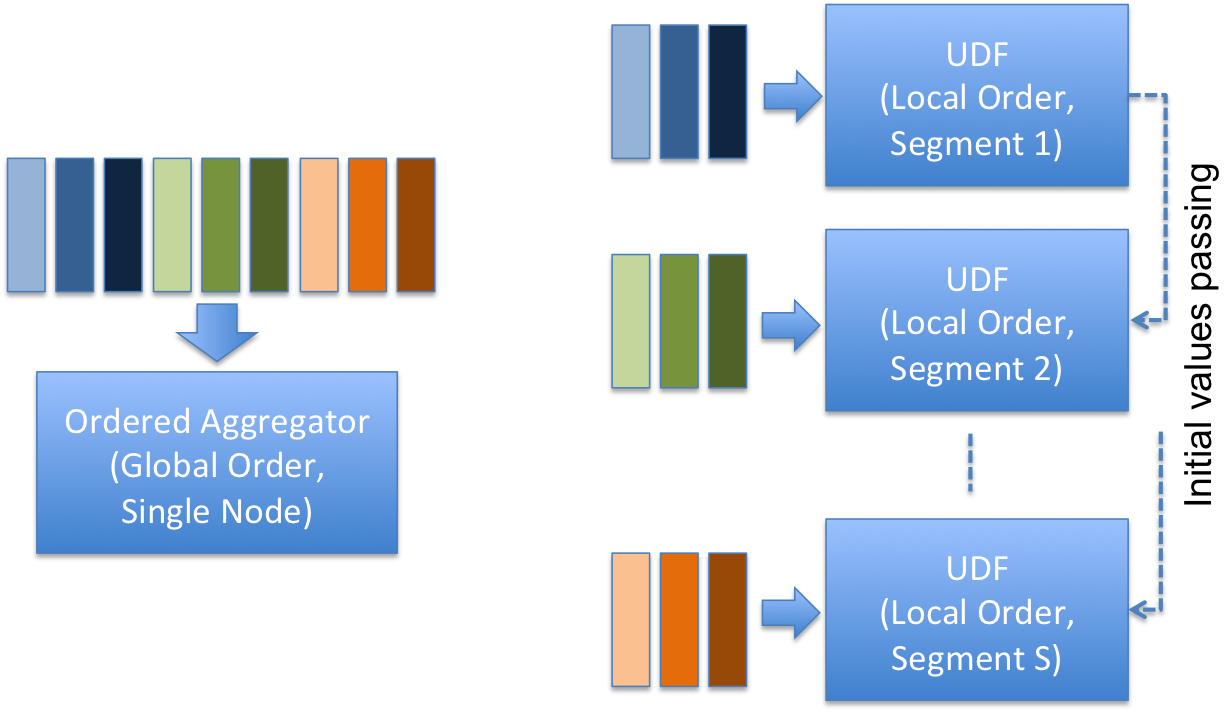
\includegraphics[width=\textwidth]{sequential_vs_distributed.png}
  \end{centering}
  \caption{\label{fig:seq_vs_dist} The comparison between sequential
    and distributed designs. A segment is a running process in parallel databases.}
\end{figure}


\subsection{What is MADlib?}

% More details on MADlib

MADlib is created by the Predictive Analytics Team at Pivotal Inc. (previously
Greenplum). It is an add-on package for Greenplum database or PostgreSQL
database. The package itself is open sourced.

Cohen et al.~\cite{mad-skills} explained that ``MAD'' stands for ``magnetic'',
``agile'', ``deep'', and ``lib'' stands for advanced (mathematical, statistical,
machine learning), parallel and scalable in-database functions.

The MADlib project was initiated in late 2010. Currently MADlib's latest
version is 1.3. By itself MADlib provides a pure SQL interface. An R
front-end named PivotalR~\cite{pivotalr} is also created by the
Predictive Analytics Team at Pivotal Inc.

MADlib can be installed and run on both Grenplum database and PostgreSQL\@. On
Greenplum database (GPDB) systems, MADlib utilizes the data parallel
funtionality. The calculation is done on multiple segments of GPDB in parallel,
and the results from the segments are summarized on the master node. In many
cases, multiple iterations of such calculations are needed. We use C++ code to
implement the part inside each iteration, which is computation intensive. We
use Python code to drive the iterations, which does not have high requirements
for the performance.

Although MADlib does not do parallel computation on PostgreSQL, it is
still valuable for process big data sets that cannot be loaded into
memory. For example, in this paper we describe our implementation of
ARIMA in MADlib. We compare our implementation 

% explain more about the C++ abstraction layer

% more about Python layer

At the time of writing, MADlib has modules for linear regression,
logistic regression, multinomial logistic regression, elastic-net
regularization for linear and logistic regressions, all kinds of
robust estimators for regressions, marginal effects, k-means,
association rules, cross validation, linear systems, matrix
factorization, LDA, data summary, correlation, hypothesis tests, SVD
and PCA, ARIMA etc and many other supporting functions.  A very
detailed user documentation is available onlin at http://madlib.net.

Here in this paper, we focus our implementation for ARIMA in MADlib.

\section{Implementation of ARIMA}

% A short summary for the next few subsections

In the next few subsections, we will first describe the algorithm that
we have used to solve the problem of maximization of partial
log-likelihood. Then, we point out the reason why it is difficult to
make the algorithm run parallel.  The difficulty is not restricted to
this specific algorithm. It is a common situation in all algorithms
that fit ARIMA models. Actually it is easy to see that many machine
learning models have similar problems. Next, we describe our solution
to this problem. Our method is quite general and can parallelize
similar problems. Then we describe a simple method to improve the
performance of our algorithm. In the end, we discuss the possible ways
to generalize our methods to other algorithms.

\subsection{The Algorithm}

% List the LM algorithm

An ARIMA model is an auto-regressive integrated moving average model. An ARIMA
model is typically expressed in the form
\begin{equation}
(1 - \phi(B)) Y_t  = (1 + \theta(B)) Z_t,
\end{equation}
where $B$ is the backshift operator. The time $t$ is from $1$ to $N$.

ARIMA models involve the following variables:
\begin{enumerate}
   \item The lag difference $Y_{t}$, where  $Y_{t} = {(1-B)}^{d}(X_{t} - \mu)$.
    \item The values of the time series $X_t$.
    \item $p$, $q$, and $d$ are the parameters of the ARIMA model.
      $d$ is the differencing order, $p$ is the order of the AR
      operator, and $q$ is the order of the MA operator.
    \item The AR operator $\phi(B)$.
    \item The MA operator $\theta(B)$.
    \item The mean value $\mu$, which is always set to be zero for
      $d>0$ or need to be estimated.
    \item The error terms $Z_t$.
\end{enumerate}

The auto regression operator models the prediction for the next
observation as some linear combination of the previous observations.
More formally, an AR operator of order $p$ is defined as
\begin{equation}
\phi(B) Y_t= \phi_1 Y_{t-1}   + \cdots +  \phi_{p} Y_{t-p}
\end{equation}

The moving average operator is similar, and it models the prediction
for the next observation as a linear combination of the errors in the
previous prediction errors.  More formally, the MA operator of order
$q$ is defined as
\begin{equation}
\theta(B) Z_t =   \theta_{1} Z_{t-1} + \cdots + \theta_{q} Z_{t-q}.
\end{equation}

We assume that
\begin{equation}
\Pr(Z_t) = \frac{1}{\sqrt{2 \pi \sigma^2}} e^{-Z^2_t/2 \sigma^2}, \quad t > 0
\end{equation}
and that  $Z_{-q+1} = Z_{-q+2} = \cdots = Z_0 = Z_1 = \cdots = Z_p =
0$. The initial values of $Y_t=X_t-\mu$ for $t=-p+1, -p+2, \dots,
0$ can be solved from the following linear equations
\begin{eqnarray}
\phi_1 Y_0 + \phi_2 Y_{-1} + \cdots + \phi_p Y_{-p+1} &=& Y_1 \nonumber\\
\phi_2 Y_0 + \cdots + \phi_p Y_{-p+2} &=& Y_2 - \phi_1 Y_1  \nonumber\\
&\vdots& \nonumber\\
\phi_{p-1} Y_0 + \phi_p Y_{-1} &=& Y_{p-1} - \phi_1 Y_{p-2} - \cdots -
\phi_{p-2} Y_1 \nonumber \\
\phi_p Y_0  &=& Y_p - \phi_1 Y_{p-1} - \cdots - \phi_{p-1} Y_{1} \label{eq:init_Y}
\end{eqnarray}

The likelihood function $L$ for $N$ values of $Z_t$  is then
\begin{equation}
L(\phi, \theta) = \prod_{t = 1}^N  \frac{1}{\sqrt{2 \pi \sigma^2}} e^{-Z^2_t/2 \sigma^2}
\end{equation}
so the log likelihood function $l$ is
\begin{eqnarray}
  l(\phi, \theta) &=& \sum_{t = 1}^N \ln \left(\frac{1}{\sqrt{2 \pi \sigma^2}}
    e^{-Z^2_t/2 \sigma^2}
  \right) \nonumber\\
  &=&  \sum_{t = 1}^N  - \ln \left( \sqrt{2 \pi \sigma^2}\right)
  -\frac{Z^2_t}{2 \sigma^2}\nonumber\\
  &=&  -\frac{N}{2} \ln \left( 2 \pi \sigma^2\right)  - \frac{1}{2
    \sigma^2} \sum_{t = 1}^N   Z^2_t\ . \label{eq:loglikelihood}
\end{eqnarray}
Thus, finding the maximum likelihood is equivalent to solving the
optimization problem (known as the conditional least squares
formation)
\begin{equation}
\min_{\theta, \phi} \sum_{t = 1}^N  Z^2_t.
\end{equation}
The error term $Z_t$ can be computed iteratively as follows:
\begin{equation}
    Z_t = X_t - F_t(\phi, \theta, \mu) \label{eq:error-terms}
\end{equation}
where
\begin{equation}
F_t(\phi, \theta, \mu) = \mu + \sum_{i=1}^p \phi_i (X_{t-i}-\mu) + \sum_{i=1}^q
\theta_i Z_{t-i}
\end{equation}

In mathematics and computing, the Levenberg-Marquardt algorithm (LMA),
also known as the damped least-squares (DLS) method, provides a
numerical solution to the problem of minimizing a function, generally
nonlinear, over a space of parameters of the function. These
minimization problems arise especially in least squares curve fitting
and nonlinear programming.

To understand the Levenberg-Marquardt algorithm, it helps to know the
gradient descent method and the Gauss-Newton method.  On many
``reasonable'' functions, the gradient descent method takes large
steps when the current iterate is distant from the true solution, but
is slow to converge an the current iterate nears the true solution.
The Gauss-Newton method is much faster for converging when the current
iterate is in the neighborhood of the true solution.  The
Levenberg-Marquardt algorithm tries to get the best of best worlds,
and combine the gradient descent step with Gauss-Newton step in a
weighted average.  For iterates far from the true solution, the step
favors the gradient descent step, but as the iterate approaches the
true solution, the Gauss-Newton step dominates.

Like other numeric minimization algorithms, LMA is an iterative
procedure.  To start a minimization, the user has to provide an
initial guess for the parameter vector, $p$, as well as some tuning
parameters $\tau$, $\epsilon_1$, $\epsilon_2$, $\epsilon_3$, and
$k_{\max}$.  Let $Z(p)$ be the vector of calculated errors ($Z_t$'s)
for the parameter vector $p$, and let $J = {(J_{1}, J_{2}, \ldots,
  J_N)}^T$ be a Jacobian matrix.

A proposed implementation is as follows:

\begin{algorithm}[ht]
  \KwIn{An initial guess for parameters $\vec{\phi}_0, \vec{\theta}_0,
    \mu_0$} \KwOut{The parameters that maximize the likelihood
    $\vec{\phi}^*, \vec{\theta}^*, \mu^*$} $k \leftarrow 0$; $v
  \leftarrow 2$; $(\vec{\phi},\vec{\theta},\mu) \leftarrow
  (\vec{\phi}_0,\vec{\theta}_0,\mu_0)$\; Calculate
  $Z(\vec{\phi},\vec{\theta},\mu)$ with Eq. (9).
  \textit{\footnotesize // Vector of errors}\; $A \leftarrow J^T J$
  \textit{\footnotesize // The Gauss-Newton Hessian approximation}\;
  $u\leftarrow \tau * \max_i(A_{ii})$ \textit{\footnotesize // Weight
    of the gradient-descent step}\; $g \leftarrow J^T
  Z(\vec{\phi},\vec{\theta},\mu)$ \textit{\footnotesize // The
    gradient descent step}\; $ \text{stop} \leftarrow (\|g\|_{\infty}
  \le \epsilon_1)$ \textit{\footnotesize // Termination Variable}\;
  \While{not stop and $k < k_{\max}$}{ $k \leftarrow k + 1$\;
    \Repeat{stop or $\rho > 0$}{ $\delta \leftarrow{(A + u \times
        \text{diag}(A))}^{-1} g$ \textit{\footnotesize // Calculate
        step direction}\; \eIf(\textit{\footnotesize // Change is too
        small to continue.})  {$\| \delta \| \le \epsilon_2 \|
        (\vec{\phi},\vec{\theta},\mu) \|$} { $\text{stop} \leftarrow
        \text{true}$\; }{
        $(\vec{\phi}_{new},\vec{\theta}_{new},\mu_{new}) \leftarrow
        (\vec{\phi},\vec{\theta},\mu) + \delta$ \textit{\footnotesize
          // A trial step}\; $\rho \leftarrow (\|
        Z(\vec{\phi},\vec{\theta},\mu)\|^2 - \|
        Z(\vec{\phi}_{new},\vec{\theta}_{new},\mu_{new})\|^2
        )/(\delta^T(u \delta + g))$ \; \eIf(\textit{\footnotesize //
          Trial step was good}){$\rho > 0$}{
          $(\vec{\phi},\vec{\theta},\mu) \leftarrow
          (\vec{\phi}_{new},\vec{\theta}_{new},\mu_{new})$
          \textit{\footnotesize // Update variables}\; Calculate
          $Z(\vec{\phi},\vec{\theta},\mu)$ with Eq. (9); $A \leftarrow
          J^T J$; $g \leftarrow J^T Z(\vec{\phi},\vec{\theta},\mu)$\;
          $ \text{stop} \leftarrow (\|g\|_{\infty} \le \epsilon_1)$ or
          $(\| Z{(\vec{\phi},\vec{\theta},\mu)}^2 \| \le \epsilon_3)$
          \; $v \leftarrow 2$; $u \rightarrow u * \max(1/3, 1 -
          {(2\rho - 1)}^3 )$\; } (\textit{\footnotesize // Trial step
          was bad}){ $v \leftarrow 2 v$; $u \leftarrow u v$\; } } } }
  $(\vec{\phi}^*,\vec{\theta}^*,\mu^*) \leftarrow
  (\vec{\phi},\vec{\theta},\mu)$\;

\label{alg:LM}
\end{algorithm}

Suggested values for the tuning parameters are $\epsilon_1 = \epsilon_2 =
\epsilon_3 = 10^{-15}, \tau = 10^{-3}$ and $k_{\max} = 100$.

The Jacobian matrix $J = {(J_{1}, J_{2}, \ldots, J_N)}^T$ requires the
partial derivatives, which are
\begin{equation}
J_t = {(J_{t, \phi_1}, \ldots, J_{t,\phi_p}, J_{t,\theta_1}, \ldots,
  J_{t,\theta_q}, J_{t,\mu})}^T
\end{equation}
Here the last term is present only when \texttt{include\_mean} is
\texttt{True}.
The iteration relations for $J$ are
\begin{eqnarray}
  J_{t, \phi_i} &=& \frac{\partial F_t(\phi,\theta)}{\partial \phi_i} =
  -\frac{\partial Z_t}{\partial \phi_i} = X_{t-i}-\mu + \sum_{j=1}^q
  \theta_j \frac{\partial Z_{t - j}}{\partial \phi_i} = X_{t-i}-\mu - \sum_{j=1}^q
  \theta_j J_{t-j,\phi_i}, \label{eq:J1}\\
  J_{t, \theta_i}&=&\frac{\partial F_t(\phi,\theta)}{\partial \theta_i} =
  -\frac{\partial Z_t}{\partial \theta_i} = Z_{t-i} + \sum_{j =1}^q
  \theta_j \frac{\partial Z_{t - j}}{\partial \theta_i} = Z_{t-i} -
  \sum_{j=1}^q \theta_j J_{t-j,\theta_i}, \label{eq:J2}\\
  J_{t, \mu} &=&\frac{\partial F_t(\phi,\theta)}{\partial \mu} =
  -\frac{\partial Z_t}{\partial \mu} = 1 -
  \sum_{j=1}^p \phi_j - \sum_{j=1}^q \theta_j \frac{\partial
    Z_{t-j}}{\partial \mu} = 1 - \sum_{j=1}^p \phi_j - \sum_{j=1}^q
  \theta_j J_{t-j,\mu}. \label{eq:J3}
\end{eqnarray}
Note that the mean value $\mu$ is considered separately in the above
formulations. When \texttt{include\_mean} is set to \texttt{False},
$\mu$ will be simply set to 0. Otherwise, $\mu$ will also be estimated
together with $\vec{\phi}$ and $\vec{\theta}$. The initial conditions
for the above equations are
\begin{equation}
J_{t,\phi_i} = J_{t,\theta_j} = J_{t,\mu} = 0 \quad \mbox{for }
t \leq p,\ \mbox{and }i=1,\dots,p; j = 1, \dots, q\ ,
\end{equation}
because we have fixed $Z_t$ for $t\leq p$ to be a constant $0$ in the
initial condition. Note that $J$ is zero not only for $t\leq 0$ but
also for $t\leq p$.

\subsection{The Problems in Parallelization}

It is very easy to see that Eqs.
(\ref{eq:error-terms},~\ref{eq:J1},~\ref{eq:J2},~\ref{eq:J3}) are
difficult to parallelize. Each step computation uses the result from
the previous step. Therefore, we have to scan through the data
sequentially to compute the quatities in these equations, and we have
to do this in every iteration. If the data set is very large then it
is time-consuming to use this algorithm. 

\subsection{Our Solution}

% Our solution and how to improve the performance

In\ order to utilize the data parallel capability of MPP database, we
propose to segment the whole time series data into a set of
consecutive time series data, numbering from $1$ to $N$, each subset
comprising a sequence of consecutive time series data of size
$K$. Since the model fitting involves multile iterations of
computations, for any subset $i$ execpt for the first one, we use the
results of the $(i-1)$-th subset from the previous iteration as the
initial values. The first subset's initial values are known. Thus in
each iteration, the computation for each subset of data does not need
to wait for the results from the previous subset. In this way, the
model fitting computaion can be parallelized. 

Besides, we find that aggregating each subset of consecutive time
series data into an array (i.e.\ a data chunk) can greatly simplify
the implementation (for example, from a stateful window function
implementation to a plain UDF implementation) and accelerate the
computation (mainly due to the reduction of I/O overhead and function
call overhead). Furthermore, we can specify the value of size $K$
according to the system configuration so that each chunk of data can
be completely loaded into the avaialble
memory. Fig. (\ref{fig:seq_vs_dist}) shows the different designs of
using a sequential implementation and a parallel implementation. 

The following SQL shows how we segment and redistribute the data
according to the above proposals.

\begin{verbatim}
create temp table dist_table as
  select
    ((tid - 1) / chunk_size)::integer + 1 as distid, 
    tid, tval
  from 
      input_table
distributed by (distid)
\end{verbatim}

The chunk size has some effect on the performance, but the effect is
not very big. 

\begin{figure}[ht]
  \begin{centering}
    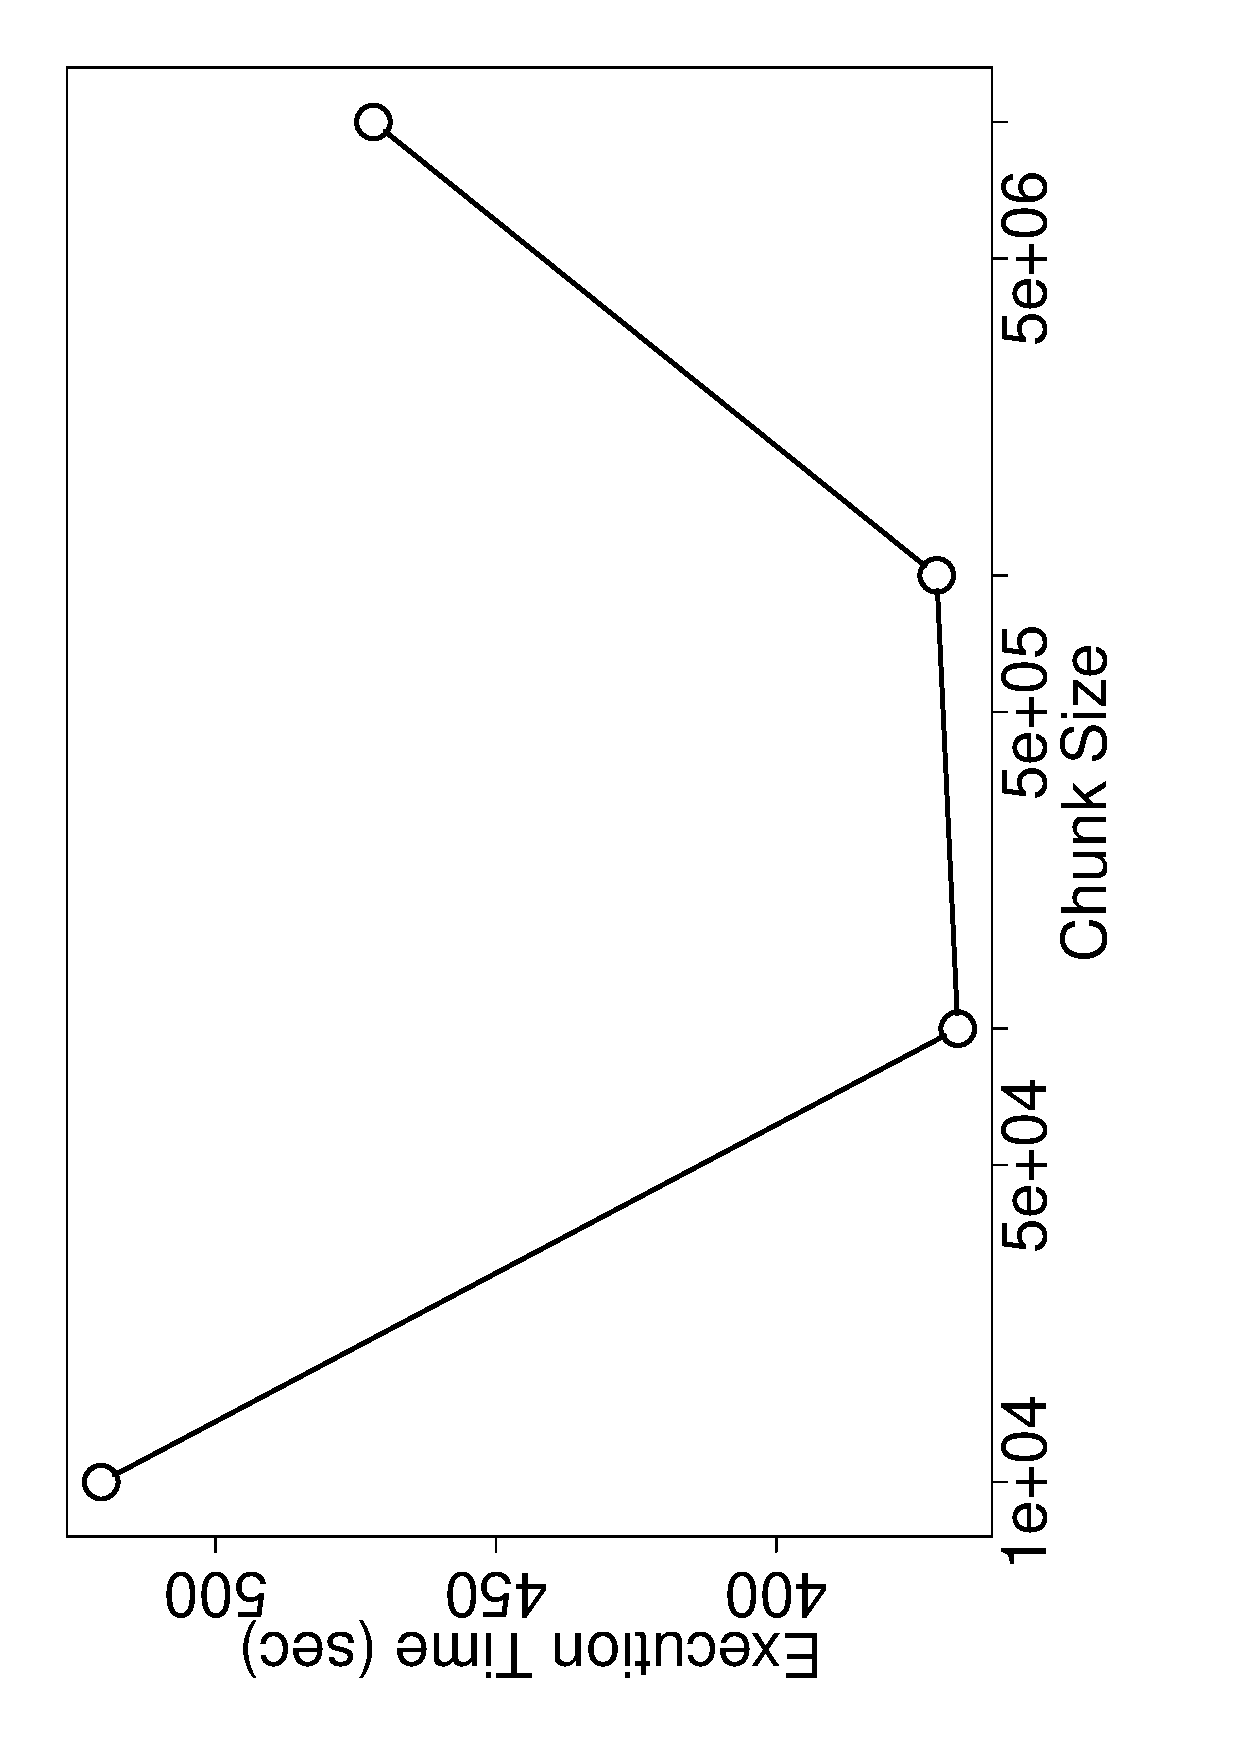
\includegraphics[angle=-90,scale=0.4]{1e8_time_vs_chunksize}
  \end{centering}
  \caption{\label{fig:chunksize_effect} We fit a time series with
    length of $10^8$ using different chunk sizes. The execution times
    are around $400$ $\sim$ $500$ secs, and are quite stable. }
\end{figure}

\begin{figure}[ht]
  \begin{centering}
    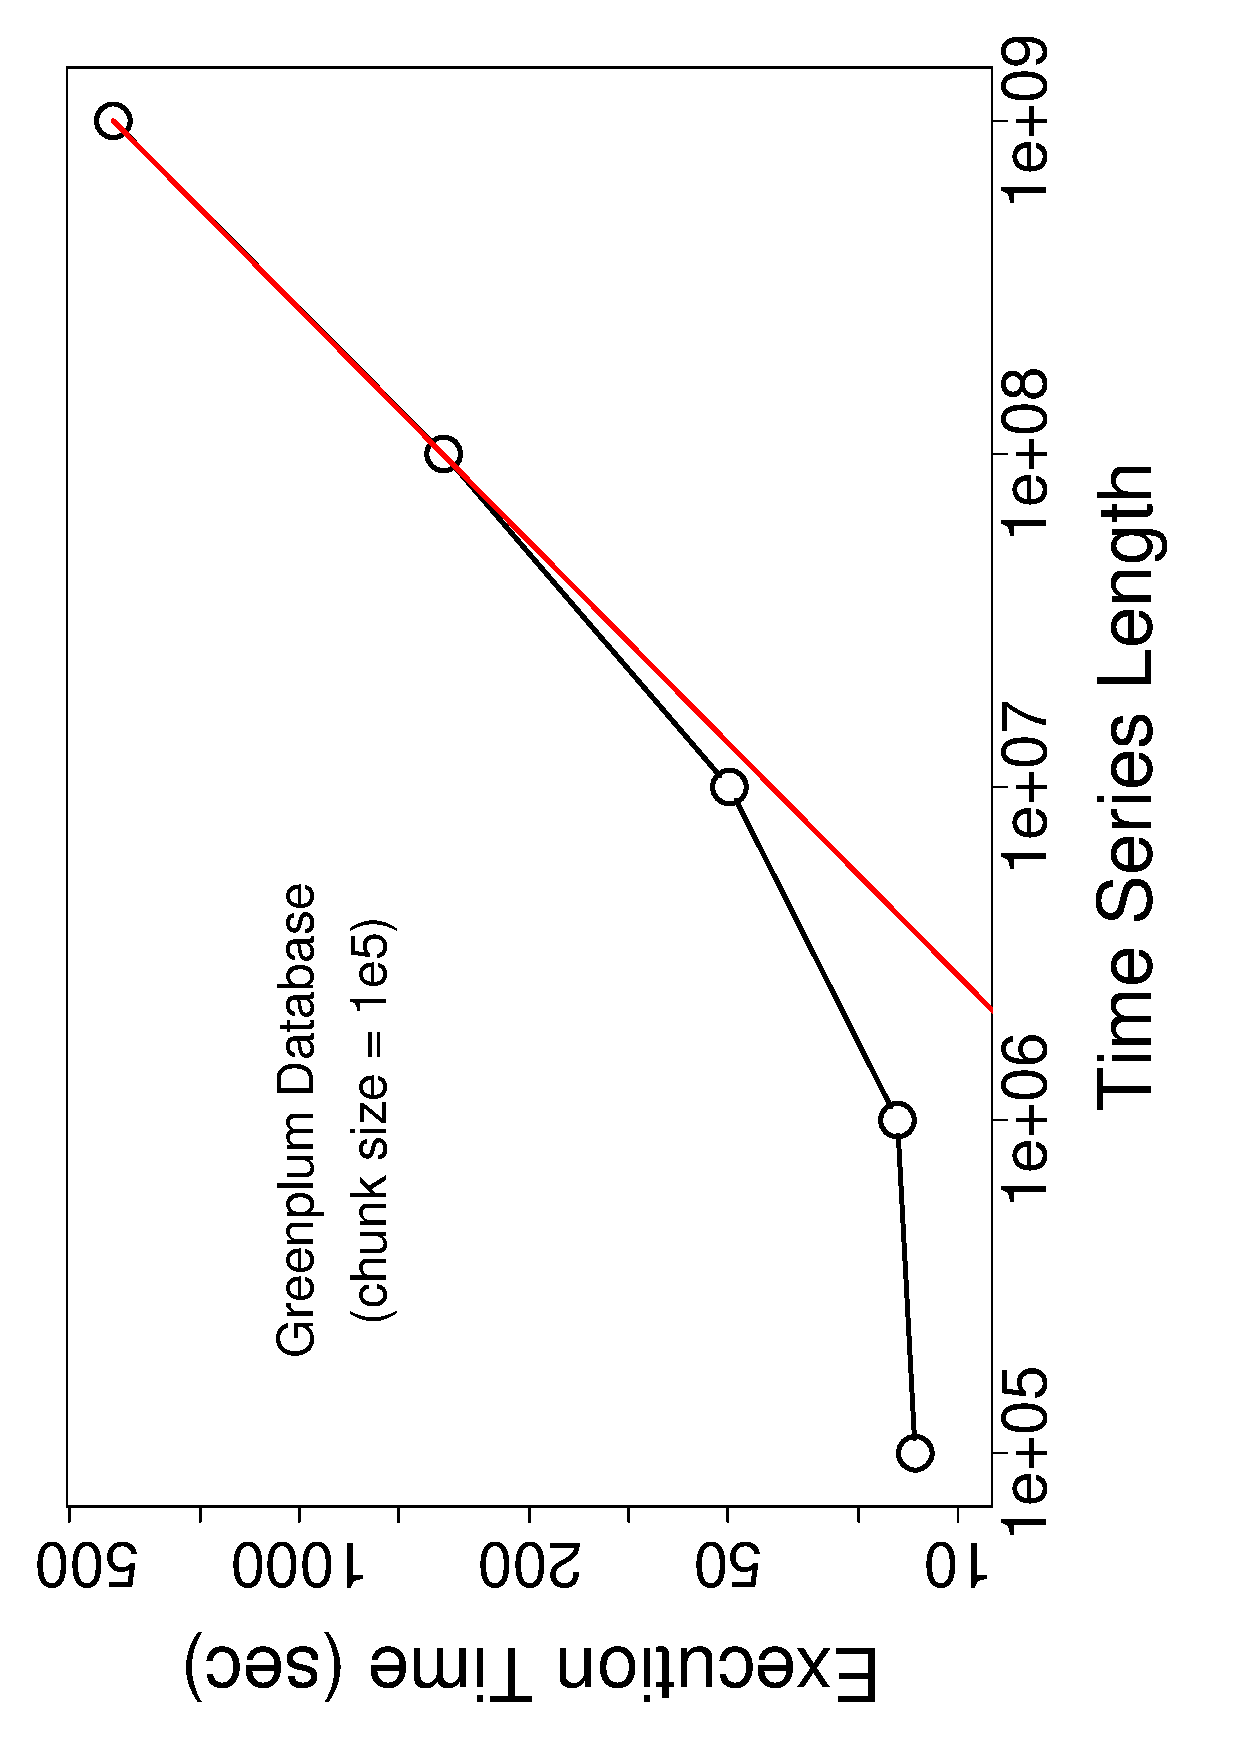
\includegraphics[angle=-90,scale=0.4]{gp_time_vs_size}
  \end{centering}
  \caption{\label{fig:gp_time_size} We fit time series with different
    lengths with the chunk size $10^5$ using MADlib's ARIMA function
    on Greenplum database. The red line is the fit to $t = \alpha l$,
    where $t$ is the execution time and $l$ is the length of the time
    series.}
\end{figure}

\begin{figure}[ht]
  \begin{centering}
    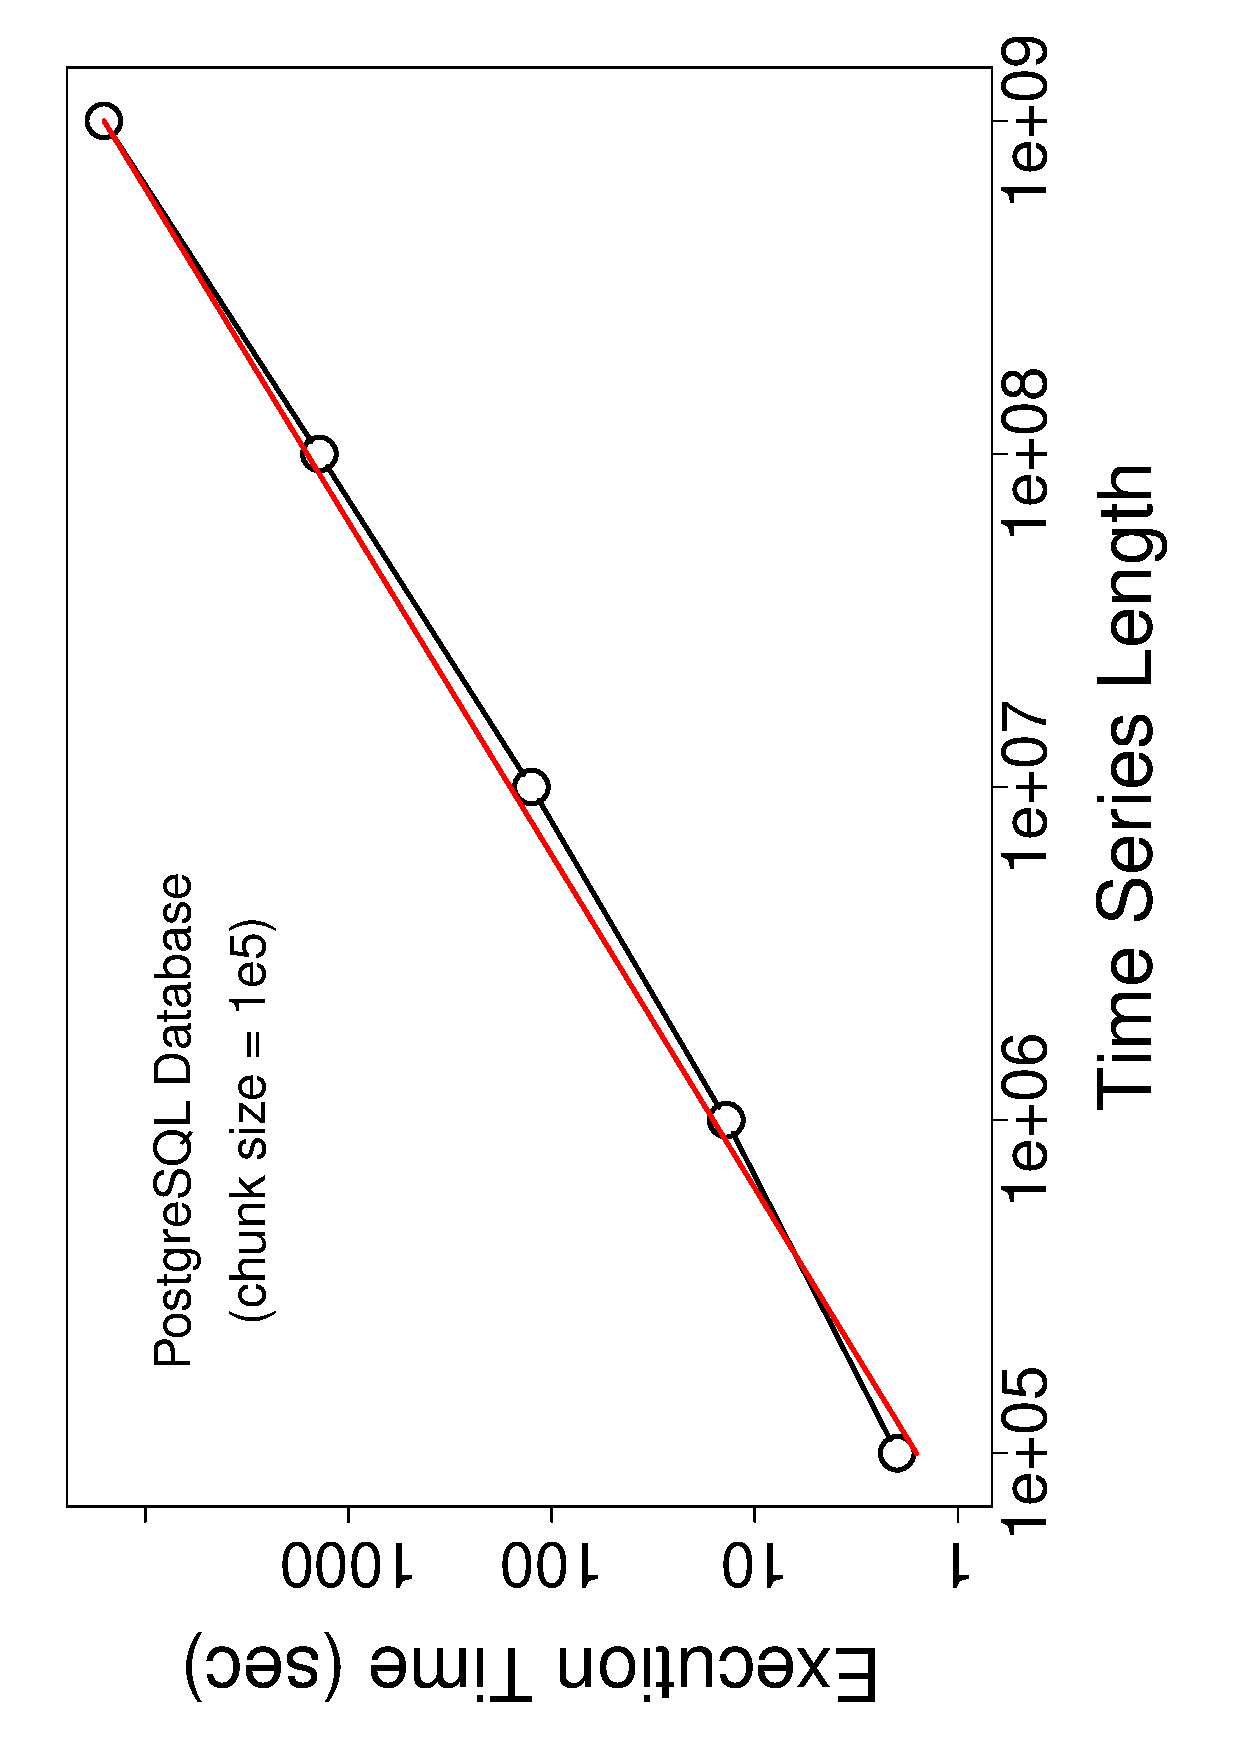
\includegraphics[angle=-90,scale=0.4]{pg_time_vs_size}
  \end{centering}
  \caption{\label{fig:pg_time_size} We fit time series with different
    lengths with the chunk size $10^5$ using MADlib's ARIMA function
    on PostgreSQL database. The red line is the fit to $t = \alpha l$,
    where $t$ is the execution time and $l$ is the length of the time
    series.}
\end{figure}

\begin{table}[ht]
  \begin{tabular}{|l|l|l|l|}
    \hline
    ~ & MADlib on GPDB & MADlib on Postgres & R's arima function \\ \hline
    Execution Time (sec) & 364.4 & 1391.9 & 1964.4 \\ \hline
  \end{tabular}
  \caption{\label{tbl:compare_R} Here we compare the execution times
    of ARIMA model fitting in R and in MADlib on Greenplum Database 
    and PostgreSQL database. The time series used to fit the ARIMA 
    model has a length of $10^8$. Note that running MADlib's ARIMA
    on Postgres is not only faster but also uses much less memory (0.1\%). 
    Running this data set in R (50G memory) uses almost 70\% of the
    machine's memory.}
\end{table}

\begin{figure}[ht]
  \begin{centering}
    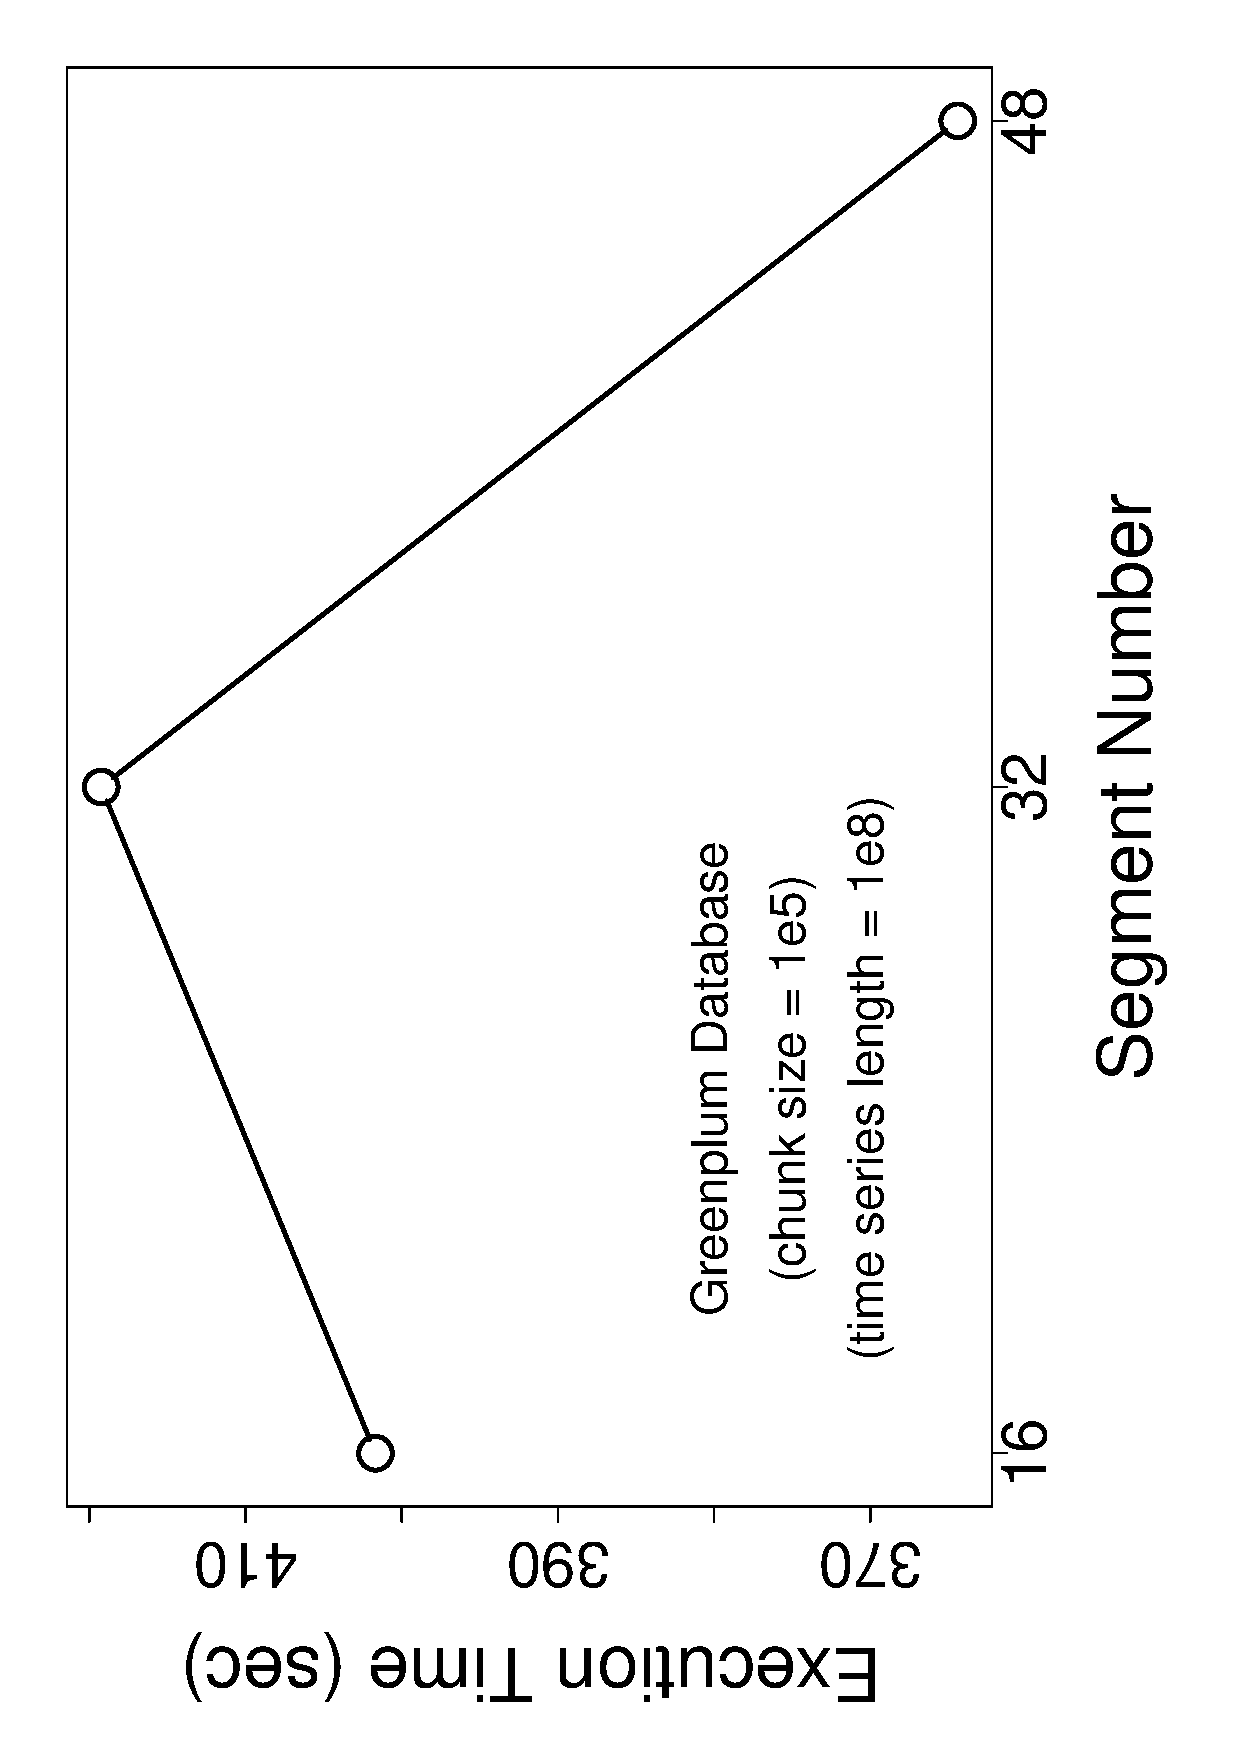
\includegraphics[angle=-90,scale=0.4]{gp_time_vs_seg}
  \end{centering}
  \caption{\label{fig:gp_time_seg} We fit a time series with length of
    $10^8$ using different numbers of segments in Greenplum database
    system.}
\end{figure}

\subsection{Performance}

% We may not be able to use Alpine's name here

Some comments about Alpine: Alpine is consistently two to threetimes
faster than MADlib on GPDB.\@ However, Alpine's result is usually very
bad if not wrong.

% Good performance improvement, some examples





\subsection{Discussion}

% Can be applied to other algorithms

\section{Conclusion}

\bibliographystyle{abbrv}

\bibliography{pred}

\end{document}
